\documentclass[12pt]{exam}

\usepackage[margin=1in]{geometry}

\newcommand{\class}{PHYS 201}
\newcommand{\term}{Spring 2013}
\newcommand{\examnum}{CO6 (v1)}
\newcommand{\examdate}{\today}
\newcommand{\timelimit}{50 Minutes}


% Engine-specific settings
% Detect pdftex/xetex/luatex, and load appropriate font packages.
% This is inspired by the approach in the iftex package.
% pdftex:
\ifx\pdfmatch\undefined
\else
    \usepackage[T1]{fontenc}
    \usepackage[utf8]{inputenc}
\fi
% xetex:
\ifx\XeTeXinterchartoks\undefined
\else
    \usepackage{fontspec}
    \defaultfontfeatures{Ligatures=TeX}
\fi
% luatex:
\ifx\directlua\undefined
\else
    \usepackage{fontspec}
\fi
% End engine-specific settings

\usepackage{amsmath,amssymb}
\usepackage{fullpage}
\usepackage{graphicx}
\usepackage[svgnames]{xcolor}
\usepackage{url}
\urlstyle{same}

\usepackage{pythontex}
% \restartpythontexsession{\thesection}


\usepackage[framemethod=TikZ]{mdframed}

\newcommand{\pytex}{Python\TeX}
\renewcommand*{\thefootnote}{\fnsymbol{footnote}}

%\usepackage{circuitikz}
\usepackage{siunitx}
\usepackage{pgfplots}
\usepackage{nopageno}



\begin{document}

%\noindent
%\begin{tabular}{l r}
%\textbf{\class} - \textbf{\examnum}  & \textbf{Name} \makebox[3.25in]{\hrulefill}  \\
%\textbf{\term} &&\\
%\textbf{\examnum} &&\\
%\textbf{\examdate} &&\\
%\textbf{Time Limit: \timelimit} & Teaching Assistant & \makebox[2in]{\hrulefill}
%\end{tabular}\\
%\rule[1ex]{\textwidth}{2.21pt}

%\pagestyle{head}
%\firstpageheader{}{}{}
%\runningheader{\class}{\examnum\ }{Page \thepage\ of \numpages}
%\runningheadrule


%\begin{questions}
%\question 


\begin{pycode}
# `from pylab import *` used to be here. It bound `uniform` to
# numpy.random.uniform while `randrange`/`randint` stayed on the standard
# library generator, so random.seed() drove only one of the two streams and
# a given paper could not be regenerated. Draw everything from one RNG.
import random

from randassign import RandAssign
ra = RandAssign()

def make_problem():
	# Random values for this problem
	def rand_mass():
		return round(random.uniform(1,3),2)
	def rand_length():
		return round(random.uniform(.5,3),2)
	def rand_speed():
		return round(random.uniform(4,8),2)
	def rand_angle():
		return random.randrange(10,65)	

		
	mass = rand_mass()
	length = rand_length()
	speed = rand_speed()
	angle = rand_angle()


		
	problem_template = r'''
    An object ($m=\SI{{{0:.3g}}}{{\kilogram}}$) is attached to one end of a string (length $=\SI{{{1:.3g}}}{{\meter}}$) having negligible mass compared to the object. The other end of the string is secured to the ceiling. \\ \\
     The speed of the object at the lowest point on its circular path is $v=\SI{{{2:.3g}}}{{\meter/\second}}$. 
    Find the object's speed at the instant when the string makes an angle of  $\theta =\ang{{{3:.3g}}} $ degrees with the vertical. \\ \\ 
    Include an energy bar chart diagram.
	'''
	
	## NO SOLUTION CODE HAS BEEN WRITTEN (YET)

	problem = problem_template.format(mass,length,speed,angle)
	
#	return(problem,V1,V2,V3,V4,I1,I2,I3,I4,W1,W2,W3,W4)
	return(problem)
	
## Generate 4 unique problems
## The chance of two identical problems is very low in this case
## But checking for identical problems won't hurt
problems = []
while len(problems) < 12:
    p = make_problem()
    if p not in problems:
        problems.append(p)
#        t = '\\SI{{{0:.3g}}}{{\\volt}} and \\SI{{{1:.3g}}}{{\\volt}}and \\SI{{{2:.3g}}}{{\\volt}} and \\SI{{{3:.3g}}}{{\\volt}} and \\SI{{{4:.3g}}}{{\\volt}} and \\SI{{{5:.3g}}}{{\\ampere}} and \\SI{{{6:.3g}}}{{\\ampere}} and \\SI{{{7:.3g}}}{{\\ampere}} and \\SI{{{8:.3g}}}{{\\ampere}} and \\SI{{{9:.3g}}}{{\\ampere}}'
#        ra.addsoln(t.format(v1,v2,v3,v4,v5,i1,i2,i3,i4,i5))

#print('\\begin{questions}')
for n, p in enumerate(problems):
    print('\\noindent \\begin{tabular}{l l r} \\textbf{\\class} - \\textbf{\\examnum}  & \\textbf{Name} \\makebox[3.25in]{\\hrulefill}  \\\\ \\end{tabular} \\\\ \\rule[1ex]{\\textwidth}{2.21pt} \\begin{questions}\\question '+ p + '\\end{questions}\\newpage')
    if n+1 < len(problems):
        print(r'\vspace{1in}')
#print('\\end{questions}')

#p = make_problem()
#t = '\\SI{{{0:.3g}}}{{\\volt}} and \\SI{{{1:.3g}}}{{\\volt}}and \\SI{{{2:.3g}}}{{\\volt}} and \\SI{{{3:.3g}}}{{\\volt}} and \\SI{{{4:.3g}}}{{\\ampere}} and \\SI{{{5:.3g}}}{{\\ampere}} and \\SI{{{6:.3g}}}{{\\ampere}} and \\SI{{{7:.3g}}}{{\\ampere}}, and \\SI{{{8:.3g}}}{{\\watt}}, and \\SI{{{9:.3g}}}{{\\watt}}, and \\SI{{{10:.3g}}}{{\\watt}} and \\SI{{{11:.3g}}}{{\\watt}}'
#ra.addsoln(t.format(v1,v2,v3,v4,i1,i2,i3,i4,w1,w2,w3,w4))

#print('\\begin{questions}\\question '+ p + '\\end{questions}')

\end{pycode}

\newpage

%\question
\noindent \begin{tabular}{l l r} \textbf{\class} - \textbf{\examnum}  & \textbf{Name} \makebox[3.25in]{\hrulefill}  \\ \end{tabular} \\ \rule[1ex]{\textwidth}{2.21pt}
\begin{questions}
  \setcounter{question}{1}
  \question Does the object in the previous question reach an angle of $\theta =\ang{90}$?  Explain why or why not. \\ \\
  Does the object reach an angle of $\theta =\ang{180}$?  Explain why or why not.

\end{questions}
\newpage

\begin{pycode}
# `from pylab import *` used to be here. It bound `uniform` to
# numpy.random.uniform while `randrange`/`randint` stayed on the standard
# library generator, so random.seed() drove only one of the two streams and
# a given paper could not be regenerated. Draw everything from one RNG.
import random

from randassign import RandAssign
ra = RandAssign()

def make_problem():
	# Random values for this problem
	def rand_mass():
		return round(random.uniform(1,3),2)
	def rand_length():
		return round(random.uniform(.5,3),2)
	def rand_speed():
		return round(random.uniform(0.15,0.45),2)
	def rand_angle():
		return random.randrange(10,65)
	def rand_k():
		return random.randrange(19,51)	

		
	mass = rand_mass()
	length = rand_length()
	speed = rand_speed()
	angle = rand_angle()
	spring = rand_k()


		
	problem_template = r'''
	A block with a mass of $m=\SI{{{0:.3g}}}{{\kilogram}}$ is placed at rest at the top of a frictionless ramp which rises at an angle,  $\theta =\ang{{{3:.3g}}} $, above the horizontal. At the top, the object is initially 8.0 m from the bottom of the incline, as shown in the figure. At the bottom of the ramp is a rough surface ($\mu_k = {2:.3g}$) that is $d = \SI{{{1:.3g}}}{{\meter}}$ long, as shown. What is not shown is a compressible spring ($k = \SI{{{4:.3g}}}{{\newton/\meter}} $).
	\\
	\\
	Determine how much the spring would need to be compressed to stop the block. Does this seem reasonable? Explain why or why not.\\ \\ 
    Include an energy bar chart diagram.
	'''
	
	## NO SOLUTION CODE HAS BEEN WRITTEN (YET)

	problem = problem_template.format(mass,length,speed,angle,spring)
	
#	return(problem,V1,V2,V3,V4,I1,I2,I3,I4,W1,W2,W3,W4)
	return(problem)
	
## Generate 4 unique problems
## The chance of two identical problems is very low in this case
## But checking for identical problems won't hurt
problems = []
while len(problems) < 12:
    p = make_problem()
    if p not in problems:
        problems.append(p)
#        t = '\\SI{{{0:.3g}}}{{\\volt}} and \\SI{{{1:.3g}}}{{\\volt}}and \\SI{{{2:.3g}}}{{\\volt}} and \\SI{{{3:.3g}}}{{\\volt}} and \\SI{{{4:.3g}}}{{\\volt}} and \\SI{{{5:.3g}}}{{\\ampere}} and \\SI{{{6:.3g}}}{{\\ampere}} and \\SI{{{7:.3g}}}{{\\ampere}} and \\SI{{{8:.3g}}}{{\\ampere}} and \\SI{{{9:.3g}}}{{\\ampere}}'
#        ra.addsoln(t.format(v1,v2,v3,v4,v5,i1,i2,i3,i4,i5))

#print('\\begin{questions}')
for n, p in enumerate(problems):
    print('\\noindent \\begin{tabular}{l l r} \\textbf{\\class} - \\textbf{\\examnum}  & \\textbf{Name} \\makebox[3.25in]{\\hrulefill}  \\\\ \\end{tabular} \\\\ \\rule[1ex]{\\textwidth}{2.21pt} \\begin{questions}\\setcounter{question}{2}\\question '+ p + '\\begin{figure}[h]\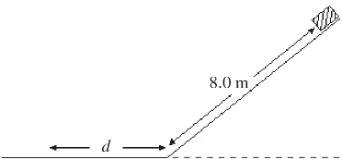
\includegraphics{Picture1}\\end{figure}\\end{questions}\\newpage')
    if n+1 < len(problems):
        print(r'\vspace{1in}')
#print('\\end{questions}')

#p = make_problem()
#t = '\\SI{{{0:.3g}}}{{\\volt}} and \\SI{{{1:.3g}}}{{\\volt}}and \\SI{{{2:.3g}}}{{\\volt}} and \\SI{{{3:.3g}}}{{\\volt}} and \\SI{{{4:.3g}}}{{\\ampere}} and \\SI{{{5:.3g}}}{{\\ampere}} and \\SI{{{6:.3g}}}{{\\ampere}} and \\SI{{{7:.3g}}}{{\\ampere}}, and \\SI{{{8:.3g}}}{{\\watt}}, and \\SI{{{9:.3g}}}{{\\watt}}, and \\SI{{{10:.3g}}}{{\\watt}} and \\SI{{{11:.3g}}}{{\\watt}}'
#ra.addsoln(t.format(v1,v2,v3,v4,i1,i2,i3,i4,w1,w2,w3,w4))

#print('\\begin{questions}\\question '+ p + '\\end{questions}')

\end{pycode}


%\end{questions}
	
\end{document}
